\setcounter{section}{11}
\section{2012 Test 1}
\begin{center}
\begin{tabular}{r | l}
	Question & Answer   \\ \hline
	1.1      & (c)      \\
	1.2      & (d)      \\
	1.3      & (d)      \\ \hline
	2.1      & (c)      \\
	2.2      & (c)      \\
	2.3      & (c) (SW) \\
	2.4      & (a) (NW) \\ \hline
	3.1      & (a)      \\
	3.2      & (d)      \\
	3.3      & (b)      \\
	3.4      & (c)      \\ \hline
	4.1      & (c) (SW) \\ \hline
	5.1      & \ref{itm:5_1_correct} \\
	5.2      & \ref{itm:5_2_correct} \\
	5.3      & \ref{itm:5_3_correct} \\ \hline
	6.1      & (a)      \\
	6.2      & (d)      \\
	6.3      & (b)      \\
	6.4      & (b) (NE) \\
	6.5      & \ref{itm:6_5_correct} \\ \hline
	7.1      & \ref{itm:7_1_correct} (NW) \\ \hline
	8.1a     &          \\
	8.1b     &          \\
	8.1c     &          \\
	8.1d     &          \\
	8.1e     &          \\
	8.1f     &          \\
	8.1g     &          \\
	8.1h     &          \\
	8.1i     &          \\
	8.1j     &          
\end{tabular}
\end{center}
\setcounter{subsection}{3}
\subsection{Problem 4}
\subsubsection{Item 1}
\begin{center}
\begin{tabular}{r | c c}
	$\delta_D                 $ & $0          $ & $1      $ \\ \hline
	$\rightarrow \{p        \}$ & $\{p,q    \}$ & $\{p  \}$ \\
	$            \{p,q      \}$ & $\{p,q,r,s\}$ & $\{p,t\}$ \\
	$       ^*\{p,      t\}$ & $\{p,q    \}$ & $\{p  \}$ \\
	$       ^*\{p,q,r,s  \}$ & $\{p,q,r,s\}$ & $\{p,t\}$
\end{tabular}
\end{center}
\setcounter{subsection}{4}
\subsection{Problem 5}
\subsubsection{Item 1}
\begin{enumerate}[label=(\alph*)]
	\item \label{itm:5_1_a} Does not accept $ababababa$
	\item \label{itm:5_1_b} Does not accept $bab$
	\item \label{itm:5_1_correct} Correct answer
	\item Incorrect because of the answers to \ref{itm:5_1_a} and \ref{itm:5_1_b} 
\end{enumerate}
\subsubsection{Item 2}
\begin{enumerate}[label=(\alph*)]
	\item \label{itm:5_2_a} Does not accept $baaba$
	\item \label{itm:5_2_b} Does not accept $bab$
	\item \label{itm:5_2_correct} Correct answer
	\item Incorrect because of the answers to \ref{itm:5_2_a} and \ref{itm:5_2_b} 
\end{enumerate}
\subsubsection{Item 3}
\begin{enumerate}[label=(\alph*)]
	\item Does not accept $bab$
	\item \label{itm:5_3_correct} Correct answer
	\item Accepts $aab$
	\item Accepts $aab$
\end{enumerate}
\setcounter{subsection}{5}
\subsection{Problem 6}
\setcounter{subsubsection}{4}
\subsubsection{Item 5}
\begin{enumerate}[label=(\alph*)]
	\item Accepts $bb$
	\item Does not accept $b$
	\item Does not accept $\varepsilon$
	\item \label{itm:6_5_correct} Correct answer
\end{enumerate}
\subsection{Problem 7}
\subsubsection{Item 1}
\begin{enumerate}[label=(\alph*)]
	\item \label{itm:7_1_correct} (NW) Correct answer
	\item (NE) Does not accept $bbab$
	\item (SW) Does not accept $\varepsilon$
	\item (SE) Does not accept $bbab$
\end{enumerate}
\subsection{Problem 8}
\subsubsection{Item 1}
\begin{enumerate}[label=(\alph*)]
	\item \textbf{False}. $\{0^n1^n\mid n \geq 0\} \in L(0^*1^*)$ and the first is not regular.
	\item \textbf{True}. Convert them to DFAs, minimize them and compare.
	\item \textbf{True}. $\{0^n0^n\mid n \geq 0\}=L((00)^*)$.
	\item \textbf{True}. Incoming to $L1$, $L2$ are connected to start nodes, outgoing are from all final nodes.
	\begin{center} 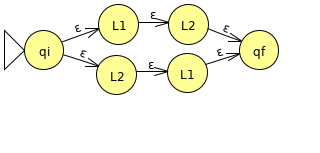
\includegraphics[scale=0.5,trim={0 20mm 0 0},clip]{2012T1_8_1d} \end{center}
	\item \textbf{False}. $\{0^n1^n\mid n \geq 0\} \cap \{01\} = \{01\}$.
	\item \textbf{False}. $(L(0^*))^*=L(0^*)$.
	\item \textbf{True}. Each state of the DFA retains the parity of $\#a$, $\#b$ and $\#c$, which requires $2^3=8$ states.
	\item \textbf{True}. These are both true because $L(a^*b^*) \subset L((a+b)^*)$.
	\item \textbf{True}. $L((a+b)^*)=\Sigma^*$ so it can be removed. Draw the DFA of $L_1$, negate it and check that it is equivalent to the righthand side.
	\item \textbf{True}. All regular languages may be represented by means of a DFA, NFA, $\varepsilon$-NFA and RE.
\end{enumerate}
